\documentclass{jdmdh}
\usepackage[utf8]{inputenc}
\usepackage{array}
\usepackage{pgfplots}
\usepackage{float}
\usepackage{tabularx}
\newcolumntype{C}{>{\arraybackslash}X} % centered "X" column


\title{Evaluating Deep Learning Methods for Tokenization of Space-less texts in Old French}
\author[1]{Thibault Clérice}
\affil[1]{École nationale des Chartes, France}
\affil[2]{Université Lyon 3, France}

\corrauthor{Thibault Clérice}{thibault.clerice@chartes.psl.eu}


\pgfplotsset{compat=1.15}
\begin{document}


\maketitle

\abstract{Tokenization of modern and old Western European languages seems to be fairly simple as it stands on the presence mostly of markers such as spaces and punctuation. Although, when dealing with old sources like manuscript written in \textit{scripta continua} or later manuscripts, (1) such markers are mostly absent, (2) spelling variation and rich morphology makes dictionary based approaches difficult. We show that applying convolutional encoding to characters followed by linear categorization to word-boundary or in-word-sequence can be used to tokenize such inputs. Additionally, we release a software with a rather simple interface for tokenizing one's corpus.}

\keywords{convolutional network; scripta continua; tokenization; Old French; word segmentation}

\section{Introduction}

% To Read : Stutzmann article.

Tokenization of space-less strings is a task that is specifically difficult for computer when compared to "whathumancando". \textit{Scripta continua} is a writing phenomenon where words are be separated by spaces and has disappeared around the 8th century (see \citet{zanna1998lecture}). Never the less, spacing can be somewhat erratic in later centuries writings, as show by Figure \ref{fig:4lines}, a document from the 13th century. In the context of text mining of HTR or OCR output, lemmatization and tokenization of medieval western languages can be a pre-processing step for further research to sustain analyses such as authorship attribution \textbf{CITE JBCAMPS ?}.

\begin{figure}[!ht]
  \centering
  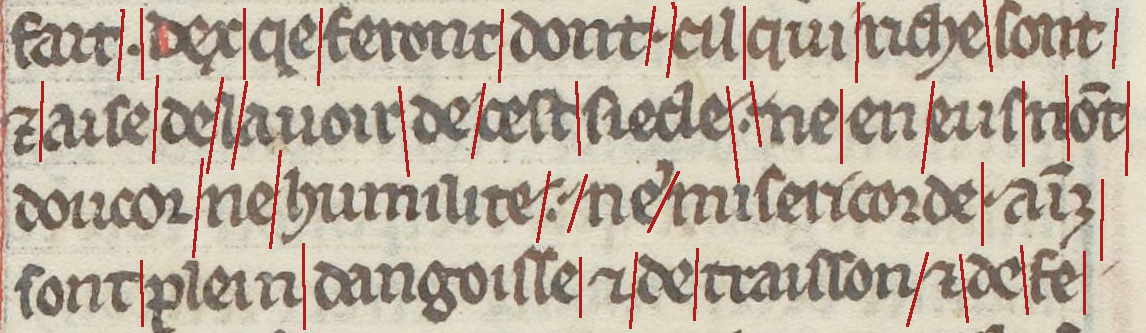
\includegraphics[width=\linewidth]{4-lines-p0215.png}

  \caption{ 4 lines from fol.103rb Manuscript fr. 412, Bibliothèque nationale de France.  Red lines indicate word boundaries}
  \label{fig:4lines}
\end{figure}

We must stress in this study that the difficulty that we face is different for \textit{scripta continua} than the ones researchers face languages such as Chinese for which an already impressive amount of work has been done as it. Indeed, Chinese word segmentation has lately been driven by deep learning methods, specifically ones based on \textit{sequence to sequence translations}: \citet{chen2015long} defines a process based on LSTM model, while \citet{yu2019learning} uses BiDirectional GRU and CRF. Actually, meanwhile redacting this article and producing the code-base, \citet{huang2019realistic} took the same approach of encoding to linear classification to both word boundary (WB) and word content (WC) for Chinese word segmentation.

Indeed, while Chinese's issue seems to lie in the decomposition of relatively fix characters, Old French or medieval latin present heavy variation of spelling. In \citet{camps_pandora}, Camps notes, in the same corpus, the existence of not less than 29 spelling of the word \textit{cheval} (horse in Old and Modern French) whose apparition counts span from 3907 to 1\footnote{These are \textit{cheval}, \textit{chevaus}, \textit{cheual}, \textit{ceval}, \textit{chevals}, \textit{cevaus}, \textit{chival}, \textit{ceual}, \textit{cheuaus}, \textit{cevals}, \textit{chaval}, \textit{chivaus}, \textit{chiual}, \textit{chevas}, \textit{cheuals}, \textit{chiuaus}, \textit{ceuaus}, \textit{chevaul}, \textit{chiuau}, \textit{chivals}, \textit{chevau}, \textit{kevaus}, \textit{chavaus}, \textit{cheuas}, \textit{keval}, \textit{cheua}, \textit{cheuau}, \textit{cheva}, \textit{chiuals}}. This  makes a dictionary approach rather difficult as it would rely on a high number of different spelling and makes the computation highly complex.

\section{Description and evaluation}

\subsection{Architecture}

\subsubsection{Encoding of input and decoding}

The model is based on traditional text input encoding where each character is transcoded to an index. Output of the model is a mask that needs to be applied to the input: in the mask, characters are classified either as word boundary or word content (\textit{cf.} Table \ref{lst:input_output_example}.

\begin{table}[!ht]
\centering
\begin{tabular}{@{}ll@{}}
\hline
                       & \textbf{Sample}           \\  \hline
\textbf{Input  String} & \texttt{Ladamehaitees'enparti}     \\
\textbf{Mask   String} & \texttt{xSxxxSxxxxxSxxxSxxxxS}     \\
\textbf{Output String} & \texttt{La dame haitee s'en parti} \\ \hline
\end{tabular}
  \caption{Input, mask and human-readable output generated by the model. x are WC and S are WB}
  \label{lst:input_output_example}
\end{table}

For evaluation purposes, and to reduce the number of input classes, we propose two options for data transcoding: a lower-case normalization and a "reduction to the ASCII character set" feature (fr. \ref{fig:normalization}). On this point, a lot of issues were found with transliteration of medieval paelographic characters that were part of the original datasets, as they are badly interpreted by the \texttt{unidecode} python package. Indeed, \texttt{unidecode} will simply remove characters it does not understand. I built a secondary package named \texttt{mufidecode} (\citet{thibault_clerice_2019_3237731}) which precedes unidecode equivalency tables when the data is known of the Medieval Unicode Font Initiative (MUFI, \citet{mufi}).

\begin{figure}[!ht]
  \centering
  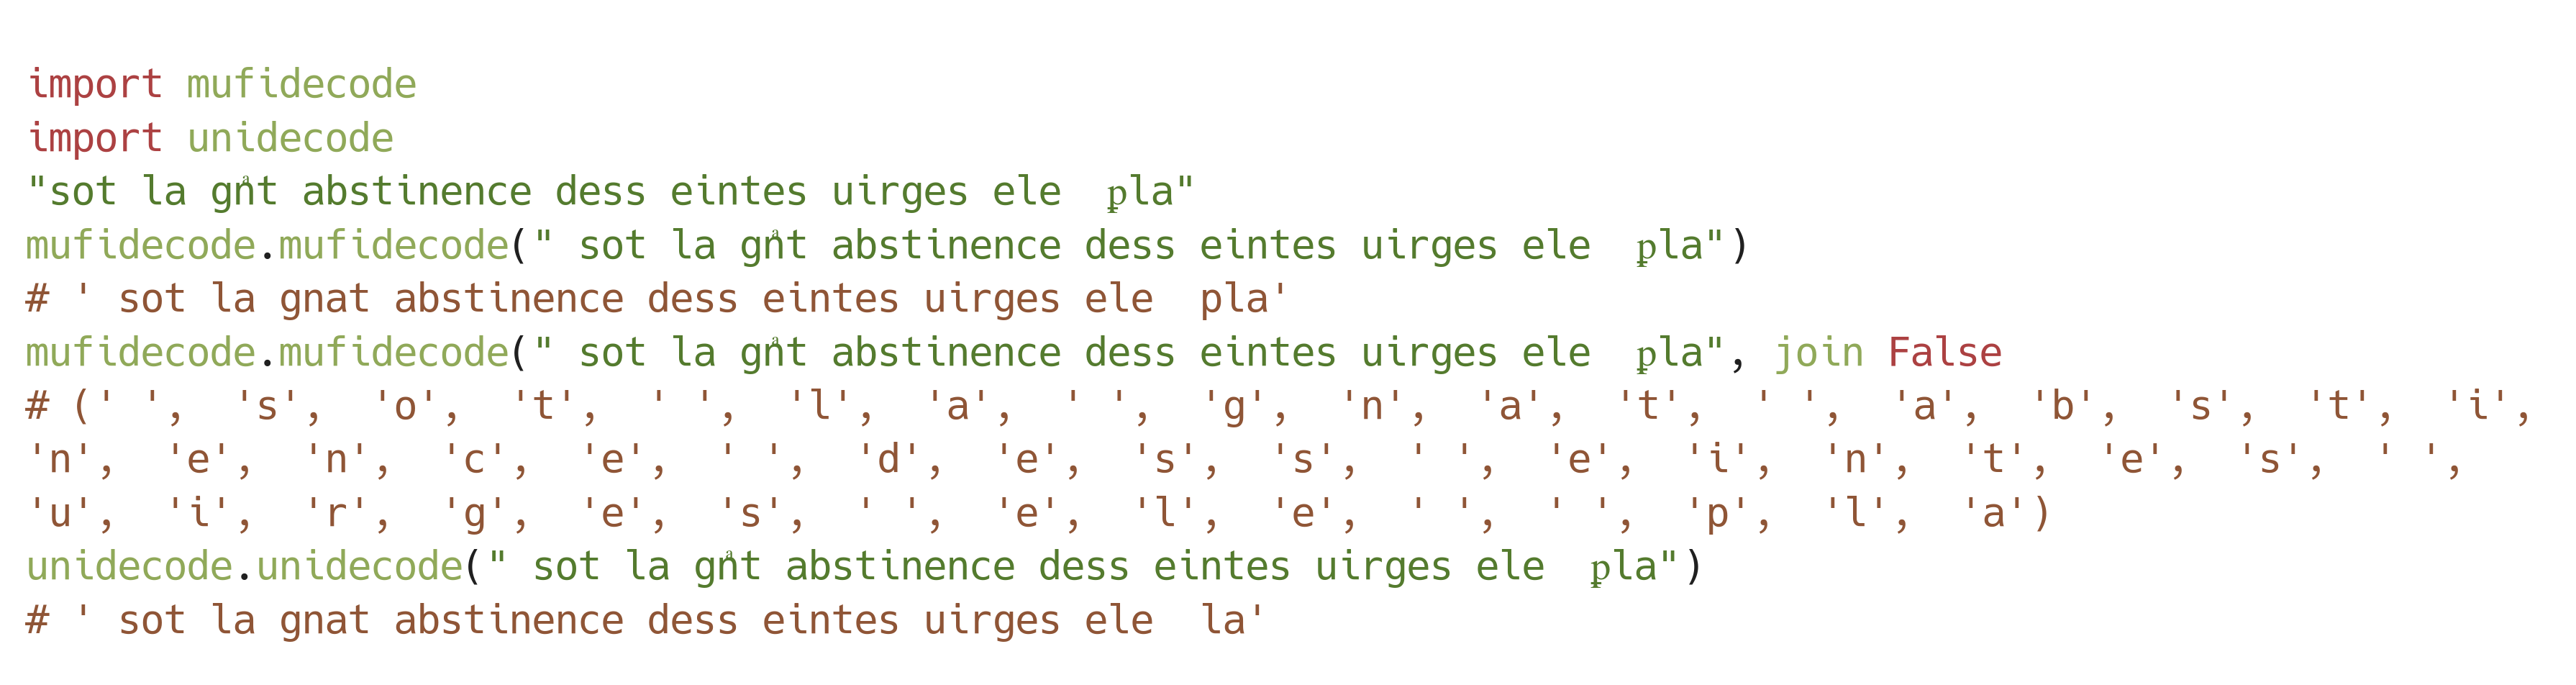
\includegraphics[width=\linewidth]{carbon.png}
  \caption{Different possibilities of pre-processing. The option with join=False was kept, as it keeps abbreviation marked as single characters. Note how \texttt{unidecode} loses the P WITH BAR}
  \label{fig:normalization}
\end{figure}

\subsubsection{Model}

Aside from normalizations of the input and output, three different structure of models were tested. Every model is composed by one encoder described below and one Linear Classifier which classifies into 5 classes : Start of Sentence (= SOS), End of Sentence (= EOS), Padding (= PAD), Masked Token (= Word Content), Space (= Word Boundary). For final scores, SOS, EOS and PAD were ignored.

The encoders are the following (configurations in parenthesis):

\begin{itemize}
  \item LSTM encoder with hidden cell (Embedding (512), Dropout(0.5), Hidden Dimension (512), Layers(10))
  \item Convolutional (CNN) encoder with position embeddings (Embedding (256), Embedding(Maximum Sentence Size=150), Kernel Size (5), Dropout(0.25), Layers (10))
  \item Convolutional (CNN) encoder without position embeddings (Embedding (256), Kernel Size (5), Dropout(0.25), Layers (10))
\end{itemize}

\subsection{Evaluation}

\subsubsection{Datasets}

Datasets are transcription from manuscripts with unresolved abbreviation coming from different projects. The \textbf{Old French} is based on \citet{8269990}, \citet{pinche:hal-01628533}, \citet{jean_baptiste_camps_2019_2630574}, \citet{bfmmss}, and \citet{tnah_transcription}. It contains

\begin{itemize}
    \item 193,734 training examples;
    \item 23,581 validation examples;
    \item 25,512 test examples
    \item Number of classes in testing examples: 482,776 WC; 169,094 WB
    \item Number of classes in unknown examples: 26,393 WC; 10,193 WB
\end{itemize}

The input was generated by grouping at least 2 words and a maximum of 8 words together per sample. On a probability of 0.2, noise character could be added (noise character was set to DOT ('.')) and some words were kept randomly from a sample to another on a probability of 0.3 and a maximum number of word kept of 1. If a minimum size of 7 characters was not met in the input sample, another word would be added to the chain. A maximum input size of 100 was kept. The results corpora should be varied in sizes as shown by \ref{fig:word_sizes}. The corpora is composed by 193 different characters when not normalized, in which some MUFI characters appears few hundred times \ref{tab:mufi_examples}.

\begin{figure}[!ht]
  \centering
  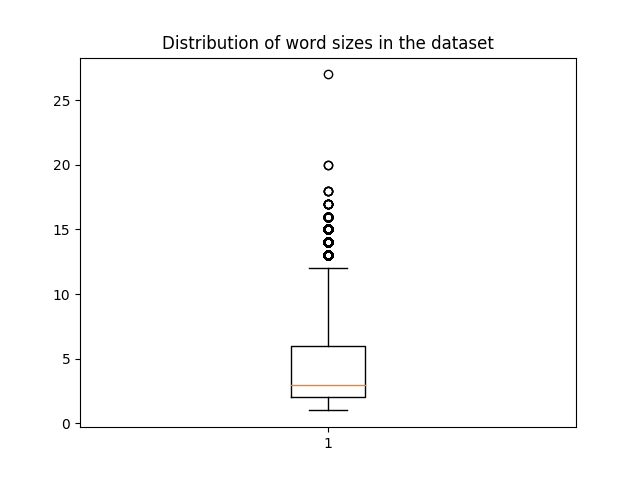
\includegraphics[width=\linewidth]{length.png}
  \caption{Distribution of word size over the train, dev and test corpora}
  \label{fig:word_sizes}
\end{figure}

\begin{table}[!ht]
\begin{tabular}{llll}
\hline
                                                   & Train dataset & Dev dataset & Test dataset \\ \hline
TIRONIAN SIGN ET                                   & 4367          & 541         & 539          \\
CON                             & 508           & 70          & 76           \\
P WITH STROKE THROUGH DESCENDER & 580           & 69          & 84           \\ \hline
\end{tabular}
  \caption{Examples of some MUFI characters distributions}
  \label{tab:mufi_examples}
\end{table}

\subsubsection{Results}

The training parameters was 0.00005 in learning rate for each CNN model and 0.001 for the LSTM one, and 64 in batch sizes. Training reached a plateau fairly quickly for each model (\textit{cf.} \ref{fig:loss}). Each model except LSTM reached a really low loss and a high accuracy on the test set (\textit{cf.} \ref{tab:scores}). To compare the results, we used the \texttt{wordsegment} package \citet{WordSegment} as a baseline.

\begin{figure}[!ht]
  \begin{center}
    \begin{tikzpicture}
      \begin{axis}[
          width=\linewidth, % Scale the plot to \linewidth
          grid=major,
          grid style={dashed,gray!30},
          xlabel=Epoch, % Set the labels
          ylabel=Accuracy,
          legend style={at={(0.5,-0.2)},anchor=north},
          x tick label style={rotate=90,anchor=east}
        ]
        \addplot table[x=Epoch,y=CNN 1,col sep=comma] {accuracies.csv};
        \addplot table[x=Epoch,y=CNN L,col sep=comma] {accuracies.csv};
        \addplot table[x=Epoch,y=CNN w/o P,col sep=comma] {accuracies.csv};
        \addplot table[x=Epoch,y=CNN N,col sep=comma] {accuracies.csv};
        \addplot table[x=Epoch,y=CNN L N,col sep=comma] {accuracies.csv};
        \legend{CNN, CNN L, CNN P, CNN N, CNN L N}
      \end{axis}
    \end{tikzpicture}
    \caption{Training Loss (Cross-entropy) until plateau was reached. N = normalized, L = Lower, P = no position embedding. LSTM was removed as it did not go below 0.65}
  \label{fig:loss}
  \end{center}
\end{figure}

\begin{table}[!ht]
\centering
\begin{tabular}{lllll}
\hline
Model    & Accuracy & Precision & Recall & FScore \\ \hline
Baseline & 0.989    & 0.986     & 0.984  & 0.985 \\
CNN      & 0.991    & 0.985     & 0.990  & 0.987  \\
CNN L    & 0.991    & 0.979     & 0.990  & 0.985  \\
CNN P    & \textbf{0.993}    & \textbf{0.990}& \textbf{0.991}  & \textbf{0.990}  \\
CNN N    & 0.991    & 0.987     & 0.988  & 0.988  \\
CNN L N  & 0.992    & 0.988     & 0.989  & 0.988  \\
LSTM     & 0.741    & 0.184     & 0.500  & 0.269  \\ \hline
\end{tabular}
\caption{Scores over the test dataset. N = normalized, L = Lower, P = no position embedding.}
\label{tab:scores}
\end{table}

\subsubsection{Unknown texts}

While all model using CNN shows improvement over the baseline, the model definitely does not outperform it by a huge margin (\textless 0.02 FScore). And for a reason : the baseline already performs nearly perfectly on the test corpus. The dictionary attack using n-grams did actually perform well. As a result, we wanted to compare how both models would perform on a secondary test corpus composed by texts that were not used in training: indeed, the training, dev and test corpus share the same texts while not sharing the same inputs. As a result, we created a new corpus with 4 texts and 742 samples : the diplomatic edition of the Graal \citet{graal}, a Passion and a Vie de Saint Leger \citet{old_french_corpus}, a Vie de Saint Thibaut \citet{theobaldus}. No noise characters and no random keeping of words were applied.

The results here were highly different (\textit{cf.} Table \ref{tab:scores_unknown}): while it appears that the CNN is able to expand its "comprehension" of the language to newer texts, the new words are more difficult to take into account for the baseline \texttt{wordsegment} n-gram approach, resulting in a respective drop to 0.945 and 0.838 FScore. WordSegment specifically performed badly with WB false positives : it had 3658 over a corpus containing 10,193 WB token (around 35 \%).

\begin{table}[!ht]
\centering
\begin{tabular}{lllllll}
\hline
 & Accuracy & Precision & Recall & FScore & WB as WC & WC as WB \\ \hline
Baseline & 0.882 & 0.893 & 0.808 & 0.838 & 3658 & 644 \\
CNN P & \textbf{0.957} & \textbf{0.948} & \textbf{0.944} & \textbf{0.945} & \textbf{854} & \textbf{723} \\ \hline
\end{tabular}
\caption{Scores over the unknown dataset. WB as WC and WC as WB are taken from the confusion matrices}
\label{tab:scores_unknown}
\end{table}

\subsubsection{Example of outputs}

The following inputs has been tagged with the CNN P model. Batch are constructed around the regular expression \texttt{\\W} with package \texttt{regex}. This explains why inputs such as \texttt{".i."} are automatically tagged as \texttt{" . i . "} by the tool. The input was stripped of its spaces before tagging, we only show the ground truth by commodity.

\begin{table}[!ht]
\centering
\begin{tabularx}{\textwidth}{|C|C|}
\hline
\textbf{Ground truth} & \textbf{Tokenized output} \\\hline
Aies joie et leesce en ton cuer car tu auras une fille qui aura .i. fil qui sera de molt grant merite devant Dieu et de grant los entre les homes.Conforte toi et soies liee car tu portes en ton ventre .i. fil qui son lieu aura devant Dieu et qui grant honnor fera a toz ses parenz. & Aies joie et leesce en ton cuer car tu auras une fille qui aura .  i .  fil qui sera de molt grant merite devant Dieu et de grant los entre les homes .  Confort e toi et soies liee car tu portes en ton ventre .  i .  fil qui son lieu aura devant Dieu et qui grant honnor fera a toz ses parenz .
\\\hline
\end{tabularx}
\caption{Output examples on a text from outside the dataset}
\label{tab:example_output}
\end{table}

\subsection{Discussion}

We believe that, aside from a graphical challenge, word segmentation in OCR from manuscripts can actually be treated from a text point of view and as a NLP task. Word segmentation for some text can be even difficult for humanist, and as such, we believe that post-processing of OCR through tools like Boudams can be a better way to achieve data-mining of the dataset.

We were surprised by the negligible effects of the different normalization methods (lower-casing; ASCII reduction; both). The presence of certain MUFI characters might provide enough information about segmentation and be in enough numbers for them not to impact the network weights.

While the baseline surprised us by performing this well on the test corpus, it definitely performed less well than the CNN on a completely unknown corpus: in this context, the proposed model actually shows its ability to carry over unknown corpora in a better way than classical ngram approaches. In light of the high accuracy of the CNN model, we believe the model should perform the same way independently from the language in Medieval Western Europe, and results in annexes on Latin confirms this for at least 2 other corpora.

\subsection{Conclusion}

Achieving 0.99 accuracy on word segmentation with a corpus as large as 25,000 test samples seems to be the first step for a more important data mining of OCRed manuscript. In aftermath, we wonder if the importance of normalization and lowering should be higher depending on the size of the corpora and its content.

\subsection{Acknowledgements}

Boudams has been made possible by two open-source repositories from which I learned and copied bits of implementation of certain modules and without which none of this paper would have been possible: \citet{enrique_manjavacas_2019_2654987} and \citet{bentrevett}. This tool was originally intended for post-processing OCR for the presentation \citet{pinchecampsclerice} at DH2019 in Utrecht.



\bibliographystyle{plainnat}
\bibliography{article}

\appendix\footnotesize

\section{Annex 1 : Confusion of CNN without position embeddings}

\begin{figure}[H]
  \centering
  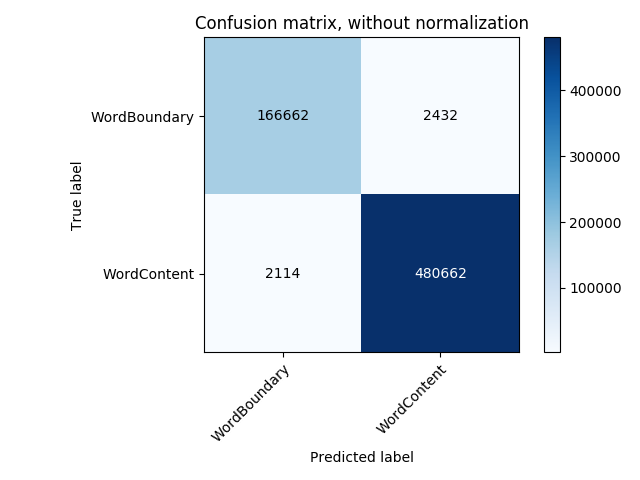
\includegraphics[width=\linewidth]{confusion.png}
  \caption{Confusion matrix of the CNN model without position embedding}
  \label{fig:confusion_matrix}
\end{figure}


\section{Annex 2 : Scores on Latin Prose and Poetic Corpora}

\begin{table}[H]
\centering
\begin{tabular}{llllllll}
\hline
 & Corpus & Accuracy & Precision & Recall & FScore & WB FN & WB FP \\ \hline
Baseline & Test & 0.978 & 0.961 & 0.974 & 0.968 & 886 & 1893 \\
CNN P & Test & \textbf{0.992} & \textbf{0.987} & \textbf{0.989} & \textbf{0.988} & \textbf{439} & \textbf{584} \\ \hline
Baseline & Unknown & 0.933 & 0.897 & 0.890 & 0.893 & 1587 & 1409 \\
CNN P & Unknown & 0.970 & 0.952 & 0.956 & 0.954 & 600 & 709 \\ \hline
\end{tabular}
\caption{Scores over the Latin classical datasets. FN = False Negative, FP = False Positive}
\label{tab:latin_corpora}
\end{table}

The Latin data is much more noisy than the Old French, as it was less curated than the digital edition we found for Old French. They are part of the Perseus corpus \citet{perseus} and were cut into passages in the context of my thesis. The training, evaluation and test corpora are built upon prose work from Cicero and Suetonius. The unknown corpus is built upon \textit{Epigrammata} from Martial, from book 1 to book 2, as it should be fairly different in word order, vocabulary, etc. Both corpus were generated without noise and word keeping, with a maximum sample size of 150 characters.

\textbf{Statistics:}
\begin{itemize}
\item Number of training examples: 30725
\item Number of evaluation examples: 3558
\item Number of testing examples: 4406
\item Number of classes in testing examples: 105,915 WC; 26,404 WB
\item Number of classes in unknown examples: 35,910 WC; 8,828 WB
\end{itemize}

\section{Annex 3: Scores on Medieval Latin corpora}

\begin{table}[H]
\centering
\begin{tabular}{llllllll}
\hline
 & Corpus & Accuracy & Precision & Recall & FScore & WB FN & WB FP \\ \hline
Baseline & Test & 0.989 & 0.981 & 0.986 & 0.982 & 1036 & 933 \\
CNN P & Test & \textbf{0.997} & \textbf{0.995} & \textbf{0.995} & \textbf{0.995} & \textbf{251} & \textbf{298} \\ \hline
Baseline & Unknown & 0.929 & 0.900 & 0.865 & 0.881 & 14,382 & 27,019 \\
CNN P & Unknown & 0.976 & 0.960 & 0.963 & 0.962 & 6509 & 7444\\ \hline
\end{tabular}
\caption{Scores over the Latin medieval datasets. FN = False Negative, FP = False Positive}
\label{tab:medieval_latin_corpora}
\end{table}

% test : 136,429+1036 WC / 933+33,120 WB
% unk  : 458,273+14,382 WC / 27,019+85,985 WB

The medieval Latin corpora is based on the project Formulae - Litterae - Chartae's open data \citet{formulae} for its training, evaluation and test sets; the unknown corpora is based on three texts from the Monumenta Germanica that are from early to late medieval period (Andreas Agnellus, Manegaldus, Theodoricus de Niem) and are drawn from the Corpus Corporum Project. Both corpus were generated without noise and word keeping, with a maximum sample size of 150 characters. The data presents some MUFI characters but still look like mostly normalized editions, unlike the Old French data.

\textbf{Statistics:}

\begin{itemize}
\item Number of training examples: 36814
\item Number of evaluation examples: 4098
\item Number of testing examples: 5612
\item Number of classes in testing examples: 137,465 WC; 34,053 WB
\item Number of classes in unknown examples: 472,655 WC; 113,004 WB
\end{itemize}

\end{document}